\section{Página principal}
\label{PPrincipal}

\begin{figure}[H]
\centerline{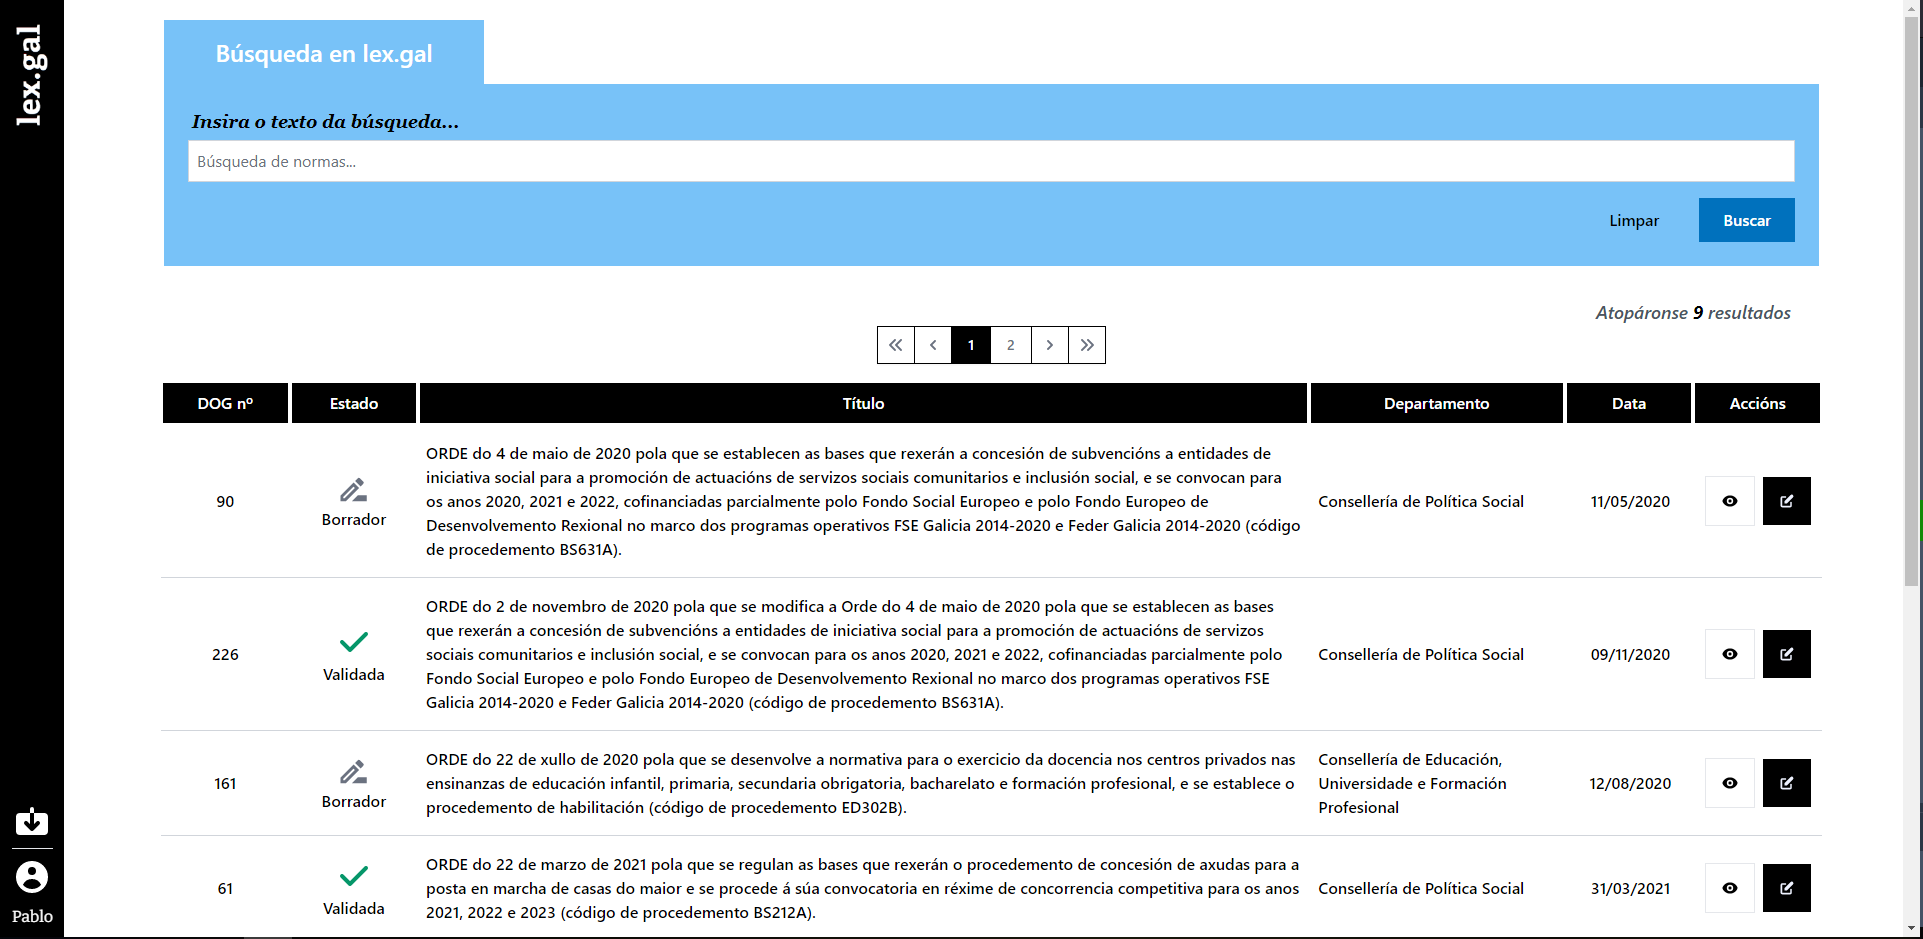
\includegraphics[width=15cm]{figuras/manualUsuario/Principal.PNG}}
\caption{Página principal/búsquedas.}
\label{enlacePPrincipal}
\end{figure}

Una vez ha sido redirigido a la página principal de la aplicación, se puede observar que se muestran todas las leyes almacenadas en la aplicación. En estas se pueden diferenciar fácilmente cinco columnas: el número del DOG, el estado (validada o borrador), el título/sumario de la ley, el departamento que lo publica, la fecha de publicación y posibles acciones a realizar. Estas acciones son: el ojo para previsualizar la ley en lex.gal (explicada en la \hyperref[PPrevisualizacionLexGal]{Sección B.5. Página de previsualización de una ley de lex.gal}), y el lápiz para editar la ley (explicada en la \hyperref[PEdicionLexGal]{Sección B.5. Página de edición de una ley de lex.gal}). 
\\

Para introducir cualquier texto que se desee buscar, se ha de insertar en el cuadro de búsqueda situado en el interior del cuadro azul. En caso de querer limpiar este texto, se puede pinchar en ``Limpar''. Además, se permite navegar entre diferentes páginas pinchando en los números situados encima y debajo de la tabla. El botón con doble flecha izquierda redirige a la primera página, y el de doble flecha derecha a la última.
\\

Si se pincha en el botón con el icono de una persona situado en la parte inferior izquierda, se abre el siguiente menú:

\begin{figure}[H]
\centerline{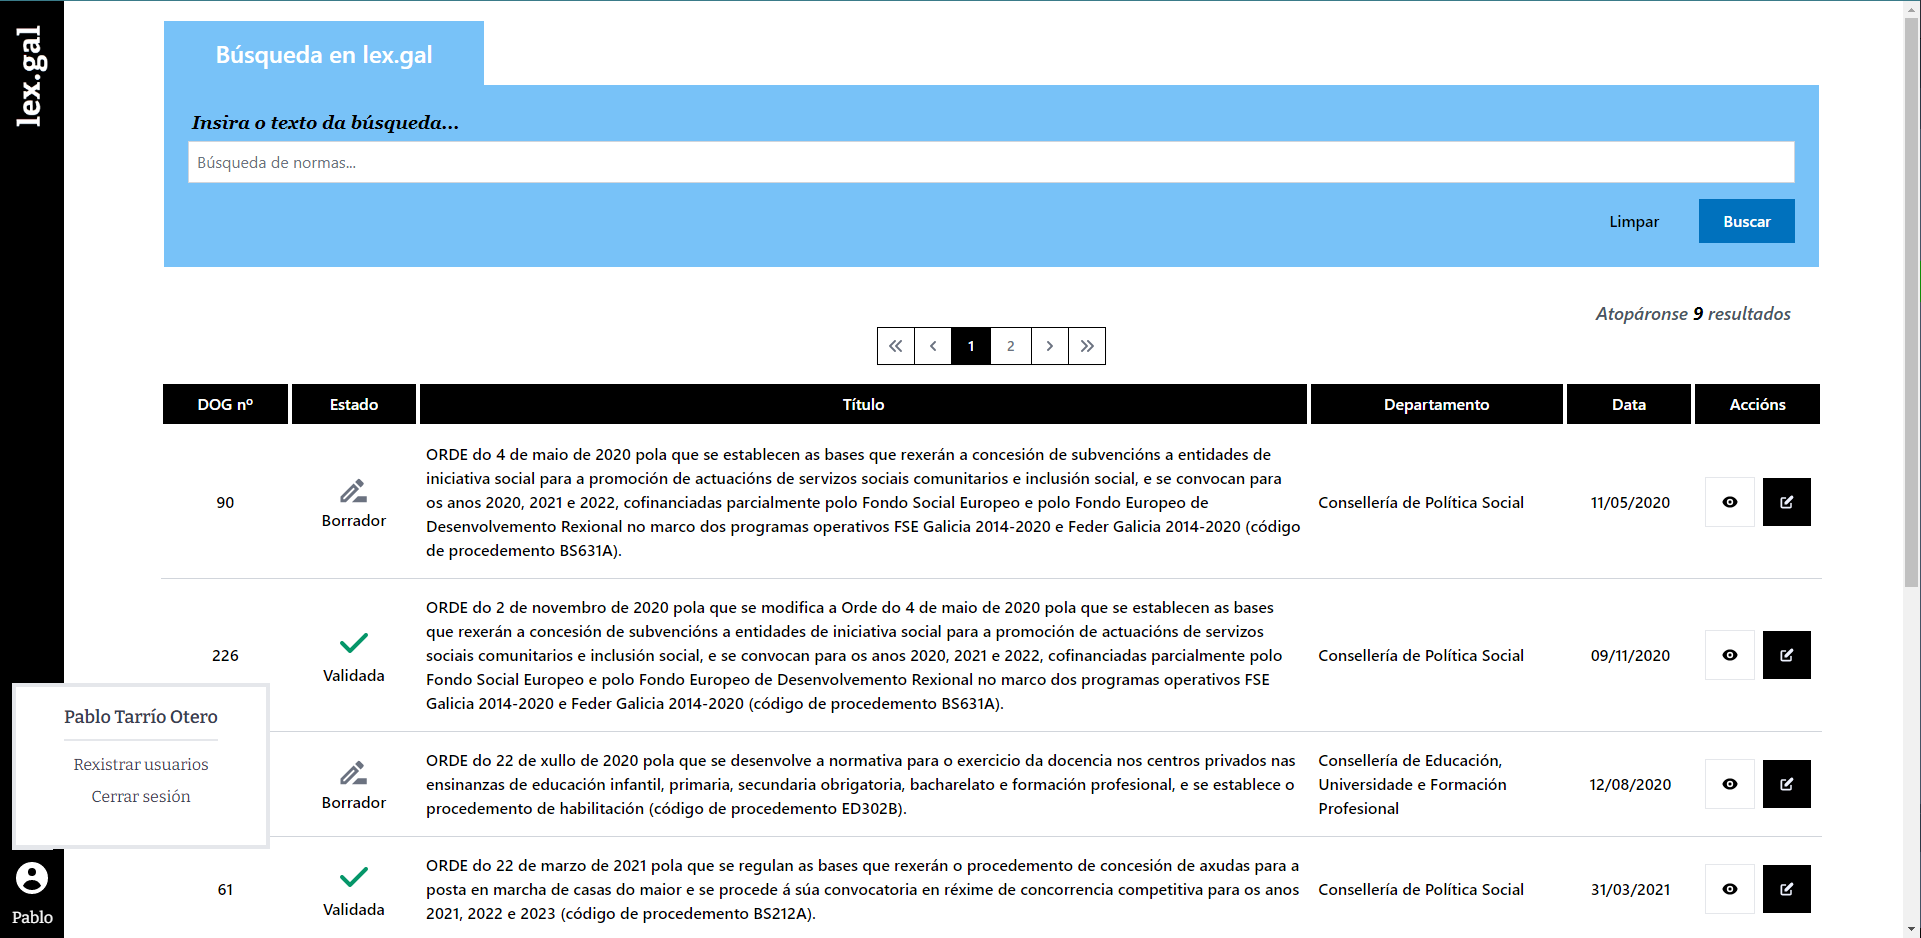
\includegraphics[width=15cm]{figuras/manualUsuario/OpcionesUsuario.PNG}}
\caption{Menú de usuarios.}
\label{enlacePMenuUsuarios}
\end{figure}

En él, se muestra el nombre de usuario y posibles acciones a realizar por este. En primer lugar, se muestra la acción de Registrar usuarios (la cual solo es visible para usuarios administradores). Si se pincha en este botón, se redirige a la página de Registro de usuarios, la cual se explica en la \hyperref[PInicioSesion]{Sección B.3. Página de registro de usuarios}. Si se pincha en el botón de Cerrar sesión, se cierra la sesión en la página y se redirige al usuario a la página de Inicio de sesión, explicada en la \hyperref[PInicioSesion]{Sección B.1. Página de inicio de sesión}.
\\

Por último, existe un último botón el cual tiene una flecha hacia abajo, y se sitúa encima del icono de la persona. Si se pincha en dicho botón, se abre una pequeña pestaña encima de la actual, la cual permitirá importar leyes del DOG, y se explica en la \hyperref[PBusquedaDOG]{Sección. B.4 Pestaña para importar del DOG}.